\begin{frame}{Quy trình xóa cuộc trò chuyện và kiểm duyệt chia sẻ}
\begin{figure}[H]
\centering
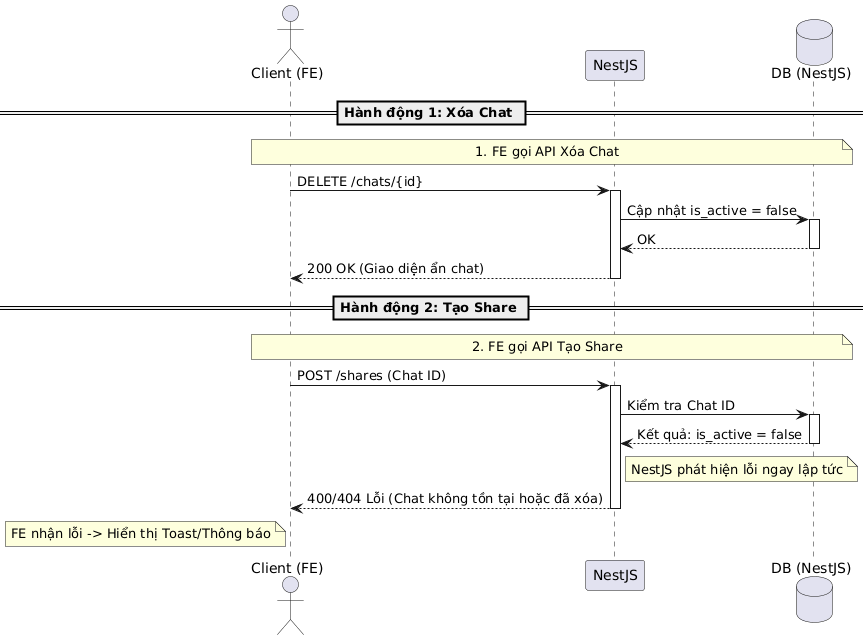
\includegraphics[height=0.55\textheight,width=0.9\textwidth,keepaspectratio]{pictures/delete-chat-validation-share.png}
\caption{Sơ đồ trình tự xóa cuộc trò chuyện và kiểm duyệt chia sẻ}
\end{figure}

\note{
Sơ đồ trình tự mô tả nghiệp vụ kiểm duyệt khi người dùng xóa cuộc trò chuyện.
Để tránh trường hợp người dùng tạo liên kết chia sẻ cho một cuộc trò chuyện đã bị xóa, hệ thống triển khai logic kiểm duyệt chặt chẽ. Khi nhận yêu cầu tạo liên kết chia sẻ, hệ thống sẽ kiểm tra trạng thái hoạt động của cuộc trò chuyện trong Database. Nếu cuộc trò chuyện đã bị xóa mềm (isActive = false), yêu cầu chia sẻ sẽ bị chặn lại và báo lỗi.
}
\end{frame}
